\documentclass[a4paper, 11pt]{article}
\usepackage{graphicx,amsmath}
\usepackage{verbatim}

\title{The \emph{xia2} manual}

\author{Graeme Winter}

\begin{document}

\maketitle
\clearpage

\tableofcontents

\section{Background}

Users of macromolecular crystallography (MX) are well served in terms of
data reduction software, with packages such as HKL2000, 
Mosflm\footnote{A.G.W. Leslie, Acta Cryst. (2006) D62, 48-57},
XDS\footnote{W. Kabsch, Acta Cryst. (2010) D66, 125-132} and 
d*TREK generally available and commonly used. In the main, however, these
programs require tha the user makes sensible decisions about the data 
analysis to ensure that a useful result is reached. This manual describes
a package, \emph{xia2}, which makes use of some of the aforementioned 
software to reduce diffraction data automatically from images to scaled 
intensities and structure factor amplitudes, with no user input.

In 2005, when the \emph{xia2} project was initiated as part of the UK BBSRC
e-Science project e-HTPX, multi-core machines were just becoming common, 
detectors were getting faster and synchrotron beamlines were becoming 
brighter. Against this background the downstream analysis (e.g. structure 
solution and refinement) was streamlined and the level of expertise needed
to use MX as a technique was reducing. At the same time mature software
packages such as Mosflm, 
Scala\footnote{P. Evans, Acta Cryst. (2006) D62, 72-82}, 
CCP4\footnote{CCP4, Acta Cryst. (1994) D50, 760-763} 
and XDS were available and a new 
synchrotron facility was being built in the UK. The ground was therefore
fertile for for the development of automated data reduction tools. Most 
crucially, however, the author was told that this was impossible and a 
waste of time - sufficient motivation for anyone.

\section{Acknowledgements}

Without the trusted and capable packes Mosflm, CCP4, Scala and XDS it would 
clearly be impossible to develop \emph{xia2}. The author would therefore
like to thank Andrew Leslie, Harry Powell, Phil Evans, Wolfgang Kabsch 
and Kay Diederichs for their assistance in using their programs and 
modifications they have made. In addition, more recent developments
such as Labelit \footnote{N.K. Sauter et al. J. Appl. Cryst. (2004) 37, 
399-409}, Pointless\footnote{P. Evans, Acta Cryst. (2006) D62, 72-82}
and CCTBX\footnote{R.W. Grosse-Kunstleve et al. J. Appl. Cryst. (2002) 35, 
126-136} have made the development of \emph{xia2} much more straightforward
and the end product. The author would therefore like to additionally thank
Nick Sauter and Ralf Grosee-Kunstleve for their help.

Development of a package such as this is impossible without test data, for
which the author would like to thank numerous users, particularly the 
Joint Centre for Structural Genomics, for publishing the majority of their
raw diffraction data. 

During the course of \emph{xia2} development the project has been 
supported by the UK BBSRC through the e-HTPX project, the EU Framework 6
through the BioXHit project and most recently by Diamond Light Source.
The software itself is open source, distributed under a BSD licence, but 
relies on the user having correctly configured and licenced the necessary
data analysis software, the details of which will be discussed shortly.

\section{Introduction}

In a nutshell, \emph{xia2} is an expert system to perform X-ray diffraction
data processing on \emph{your} behalf, using \emph{your} software with little
or no input from \emph{you}. It will correctly handle multi-pass, 
multi-wavelength data sets as described later but crucially it is not a
data processing package. Specifically, if you use \emph{xia2} in published
work please include the references for the programs it has used, which are
printed at the end of the output.

The system was initially written to support remote access to synchrotron 
facilities, however it may prove useful to anyone using MX, for example:

\begin{itemize}
\item{assisting new or novice users,}
\item{giving a second opinion to experts,}
\item{assisting busy users to allow them to focus on problem cases, or}
\item{providing reproducible processing.}
\end{itemize}

\noindent
The last of these may be most useful for users in a pharmacutical setting,
or people wishing to test or benchmark equipment, for example beamline 
scientists. In all cases however the usage of the program is the same.

\section{Using xia2}

\begin{center}
\begin{tabular}{c}
{\huge
xia2 -2d /here/are/my/data
}\\
\\
{\huge \emph{- or -}} \\
\\
{\huge
xia2 -3d /here/are/my/data
}\\
\end{tabular}
\end{center}

The program is used from the command-line, there is no GUI. In essence there
are four command-line options which are useful on a daily basis:

\begin{itemize}
\item{-atom X - tell xia2 to separate anomalous pairs i.e. $I(+) \ne I(-)$ in 
scaling}
\item{-2d - tell xia2 to use MOSFLM and SCALA}
\item{-3d - tell xia2 to use XDS and XSCALE}
\item{-3dii - tell xia2 to use XDS and XSCALE, indexing with peaks found from
all images}
\end{itemize}

\noindent
These specify in the broadest possible terms to the program the manner in
which you would like the processing performed. The program will then read all 
of the image headers found in \verb|/here/are/my/data| to organise the data, 
first into sweeps, then into wavelengths, before assigning all of these
wavelengths to a crystal.

[FIXME FIGURE]

The data from the experiment is understood as follows. The SWEEP, which 
corresponds to one ``scan,'' is the basic unit of indexing and integration.
These are contained by WAVELENGTH objects which correspond to CCP4 MTZ 
datasets, and will ultimately have unique Miller indices. For example, a low
and high dose pass will be merged together. A CRYSTAL however contains all 
of the data from the experiment and is the basic unit of data for scaling.

\begin{figure}
{\small
\begin{verbatim}
BEGIN PROJECT AUTOMATIC
BEGIN CRYSTAL DEFAULT

BEGIN HA_INFO
ATOM Ba
END HA_INFO

BEGIN WAVELENGTH SAD
WAVELENGTH 0.979500
END WAVELENGTH SAD

BEGIN SWEEP SWEEP1
WAVELENGTH SAD
DIRECTORY /dls/i02/data/2011/mx1234-5
IMAGE K5_M1S3_3_001.img
START_END 1 450
END SWEEP SWEEP1

END CRYSTAL DEFAULT
END PROJECT AUTOMATIC
\end{verbatim}
}
\caption{The input file to the program, which is generated automatically, shows
how the input data are understood. This may be adjusted and the program rerun,
which will be covered in more detail later in the manual.}
\end{figure}

\section{Introductory example}

The most straightforward way to discuss the operation of the program is 
through demonstrations with real examples. The first of these is a DNA / 
ligand complex recorded at Diamond Light Source as part of ongoing research.
The structure includes barium which may be used for phasing, and the data
were recorded as a single sweep. As may be seen from [FIXME FIGURE] the
quality of diffraction was not ideal, and radiation damage was an issue.
Initially the data were processed with 

\begin{center}
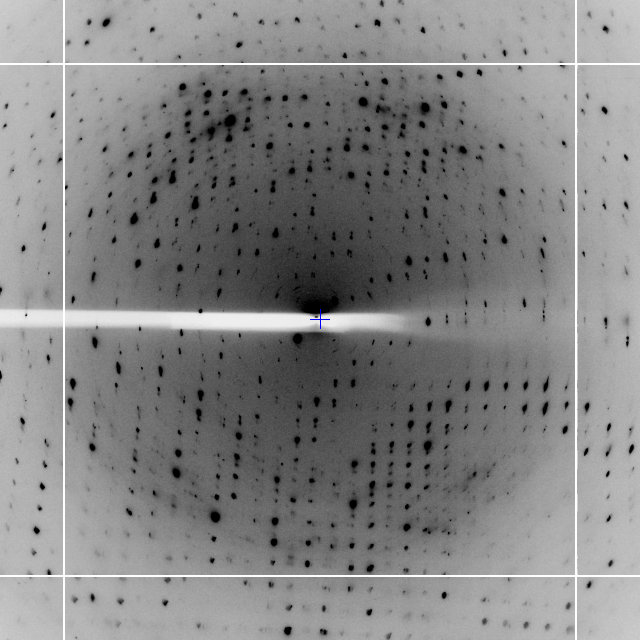
\includegraphics[scale=0.35]{figures/3qrn-diffraction.png}
\end{center}

\begin{center}
{\huge
xia2 -3d -atom Ba /here/are/my/data
}
\end{center}

\noindent
giving the merging statistics shown in [FIXME TABLE]. From these it is clear
that there is something wrong: it is very unusual to have near atomic 
resolution diffraction with $\sim 10\%$ $R_{\rm{merge}}$ in the low resolution
bin. The most likely reasons are incorrect assignment of the pointgroup and
radiation damage - the latter of which is clear from the analysis of 
$R_{\rm{merge}}$ as a function of image number [FIXME FIGURE.] A development 
option is now available (-3da rather than -3d) which will run Aimless in the 
place of Scala for merging, and which gives the cumulative completeness as
a function of frame number, as shown in FIXME FIGURE. From this it is clear 
that the data were essentially complete after approximately 200 frames. 

\begin{tabular}{lccc}
High resolution limit      &       1.25 &    6.45 &   1.25\\
Low resolution limit       &                18.85  & 18.85  &  1.27\\
Completeness               &                95.2   & 60.1  &  70.2\\
Multiplicity               &               12.2    & 8.4   &  4.8\\
I/sigma                    &               12.3    & 18.5   &  2.6\\
Rmerge                     &             0.113  & 0.096 &  0.564\\
Rmeas(I)                   &             0.129  & 0.118 &  0.633\\
Rmeas(I+/-)                &             0.121  & 0.105 &  0.679\\
Rpim(I)                    &             0.034  & 0.038 &  0.267\\
Rpim(I+/-)                 &             0.043  & 0.041 &  0.368\\
Wilson B factor            &            12.131& & \\
Anomalous completeness     &            93.3  &  52.6  &  58.0\\
Anomalous multiplicity     &           6.4    & 5.0  &   2.0\\
Anomalous correlation      &            0.544 &  0.791 & -0.297\\
Anomalous slope            &      1.085 &  0.000 &  0.000\\
Total observations         &       118588 & 529  &   1634\\
Total unique               &         9749  &  63 &     337\\
\end{tabular}

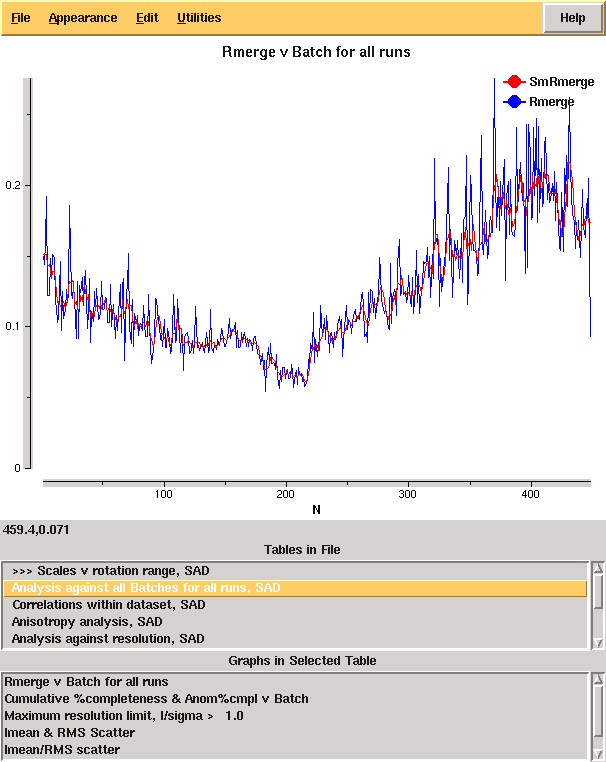
\includegraphics[scale=0.25]{figures/3qrn-all-rmerge-aimless.png}
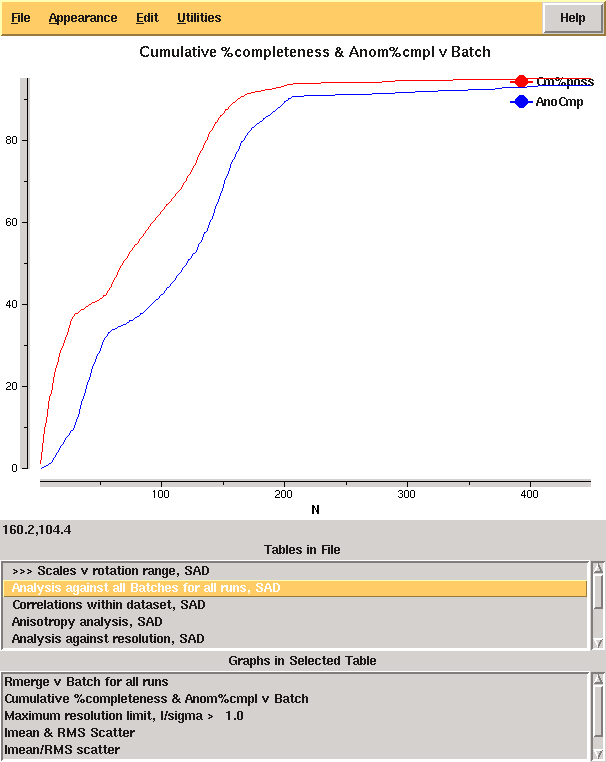
\includegraphics[scale=0.25]{figures/3qrn-all-complete-aimless.png}

\subsection{Modifying input}

From the example it would seem sensible to investigate processing only the
first 200 of the 450 images. While it is usual to limit the batch range in 
scaling when processing the data manually, \emph{xia2} is not set up to 
work like this as decisions made for the full data set (e.g. scaling model
to use) may differ from those for the subset - we therefore need to rerun the
whole \emph{xia2} job after modifying the input. All that is necessary is to 
adjust the image range (START\_END) to get the modified input file shown in 
FIXME FIGURE and rerun as 

\begin{center}
{\huge
xia2 -3d -xinfo modified.xinfo
}
\end{center}

\noindent
giving the results shown in FIXME TABLE. These are clearly much more internally
consistent and give nice results from experimental phasing. At the same time 
we may wish to adjust the resolution limits to give more complete data in the 
outer shell, which may be achieved by adding a RESOLUTION instruction to 
either the SWEEP or WAVELENGTH block.

\begin{verbatim}
BEGIN PROJECT AUTOMATIC
BEGIN CRYSTAL DEFAULT

BEGIN HA_INFO
ATOM Ba
END HA_INFO

BEGIN WAVELENGTH SAD
WAVELENGTH 0.979500
END WAVELENGTH SAD

BEGIN SWEEP SWEEP1
WAVELENGTH SAD
DIRECTORY /dls/i02/data/2011/mx1234-5
IMAGE K5_M1S3_3_001.img
START_END 1 200 ! THIS WAS 450
END SWEEP SWEEP1

END CRYSTAL DEFAULT
END PROJECT AUTOMATIC
\end{verbatim}

\begin{tabular}{lccc}
High resolution limit         &         1.22 &  6.34 &  1.22 \\
Low resolution limit          &        19.62 & 19.62 &  1.24 \\
Completeness                  &         86.9 &  49.1 &  37.8 \\
Multiplicity                  &        5.3  &  4.9   & 1.7 \\
I/sigma                       &        20.1 &  37.0  &  2.3 \\
Rmerge                        &       0.036 & 0.020  &0.355 \\
Rmeas(I)                      &       0.060 & 0.038  &0.448 \\
Rmeas(I+/-)                   &       0.043 & 0.023  &0.491 \\
Rpim(I)                       &       0.023 & 0.014  &0.297 \\
Rpim(I+/-)                    &       0.022 & 0.011  &0.339 \\
Wilson B factor               &       10.70& \\
Anomalous completeness        &        77.7  & 41.0  & 18.3 \\
Anomalous multiplicity        &         2.7  &  3.5  &  0.5 \\
Anomalous correlation         &        0.779 & 0.931 & 0.000 \\
Anomalous slope               &       1.553  &0.000 & 0.000 \\
Total observations            &       50875  &272   & 342 \\
Total unique                  &       9552   &55    & 199 \\
\end{tabular}

\section{Program Output}

As the program runs the key results are written to the screen and recorded
in the file \verb|xia2.txt|. This includes everything you should read and
includes appropriate citations for the programs that \emph{xia2} has used
on your behalf. There is also a file \verb|xia2-debug.txt| 
which should be send to 
xia2.support@gmail.com in the event of program failure. There are also two 
sensibly named directories, \verb|LogFiles| and \verb|DataFiles|, which will
be discussed shortly.

\subsection{xia2.txt}

In intention of the program output from \emph{xia2} is that it includes only
the information which is critical to read, as will be shown for a 450 image 
Pilatus 2M data set recorded from a Thaumatin crystal. Tthe results from 
indexing are displayed as lattice / unit cell:

{\small
\begin{verbatim}
------------------- Autoindexing SWEEP1 --------------------
All possible indexing solutions:
tP  57.60  57.60 149.51  90.00  90.00  90.00
oC  81.45  81.46 149.51  90.00  90.00  90.00
oP  57.59  57.60 149.50  90.00  90.00  90.00
mC  81.46  81.45 149.50  90.00  89.95  90.00
mP  57.60  57.59 149.53  90.00  89.93  90.00
aP  57.59  57.61 149.52  89.93  89.99  89.99
Indexing solution:
tP  57.60  57.60 149.51  90.00  90.00  90.00
\end{verbatim}
}

\noindent
where in each case the solution with the lowest penalty is displayed. The 
results of integration are displayed as one character per image - which 
allows the overall behaviour of the data to be understood at a glance. While
mostly 'o' is usually a good indication of satisfactory processing, '\%'
are not unusual, along with '.' for weaker data. If the output consists
of mostly 'O' then it may be helpful to record a low dose data set. The output
looks like:

{\small
\begin{verbatim}
-------------------- Integrating SWEEP1 --------------------
Processed batches 1 to 450
Weighted RMSD: 0.26 (0.09)
Integration status per image (60/record):
ooooooooooooooooooooooooooooooooooo.oooooooooooooooooooooooo
ooooooooooooooooooooooo.ooooooooooooooooooo.ooooooo.oooooooo
ooo.o.ooooooo.oooooooooooooooooooooooooooooooooooooooooooooo
oooooooooooooooooooooooooooooooooooooooooooooooooooooooooooo
oooooooooooooooooooo.ooooooooooooooooooooooooooooooooooooooo
ooooooooooooooooooooooooooooooooooooooooooooooooooo.oooooooo
ooooooooo.oooooooooo..ooo.oooooooooooooooooooo.ooooooooooooo
oooooooooooooooooooo.oooooooo.
"o" => good        "%" => ok        "!" => bad rmsd
"O" => overloaded  "#" => many bad  "." => blank
"@" => abandoned
Mosaic spread: 0.140 < 0.189 < 0.290
\end{verbatim}
}

\noindent
and includes a convenient legend.

\section{Commonly used program options}

There are a number of program options which are used on a daily basis in 
\emph{xia2}, which are:

\begin{itemize}
\item{-atom X - tell xia2 to separate anomalous pairs i.e. $I(+) \ne I(-)$ in 
scaling}
\item{-2d - tell xia2 to use MOSFLM and SCALA}
\item{-3d - tell xia2 to use XDS and XSCALE}
\item{-3dii - tell xia2 to use XDS and XSCALE, indexing with peaks found from
all images}
\item{-xinfo modified.xinfo - use specific input file}
\item{-image /path/to/an/image.img - process specific scan}
\item{-spacegroup spacegroup\_name - set the spacegroup, e.g. P21}
\item{-cell a,b,c,$\alpha$,$\beta$,$\gamma$ - set the cell constants} 
\item{-small\_molecule - don't run things like TRUNCATE}
\end{itemize}















\section{Installing xia2}

\section{Undocumented features}








\section{What did it do?}

\begin{center}
\Huge What did it do? and why?
\end{center}

\subsection{Indexing}
\begin{itemize}
\item{Initial indexing with LABELIT from 3 images\footnote{This is \emph{not}
good for small molecule data}}
\item{Refine results with XDS indexing}
\item{Use data based on general analysis @ 0, 45, 90 degrees}
\end{itemize}

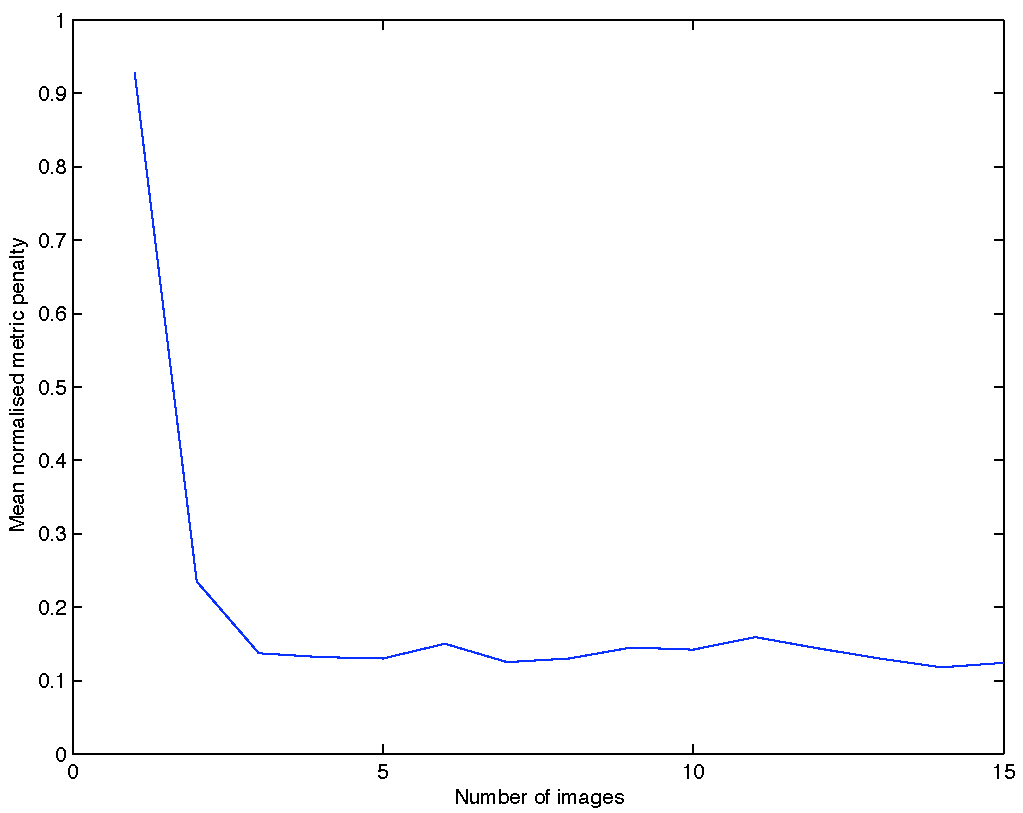
\includegraphics[scale=0.5]{figures/no_images.pdf}
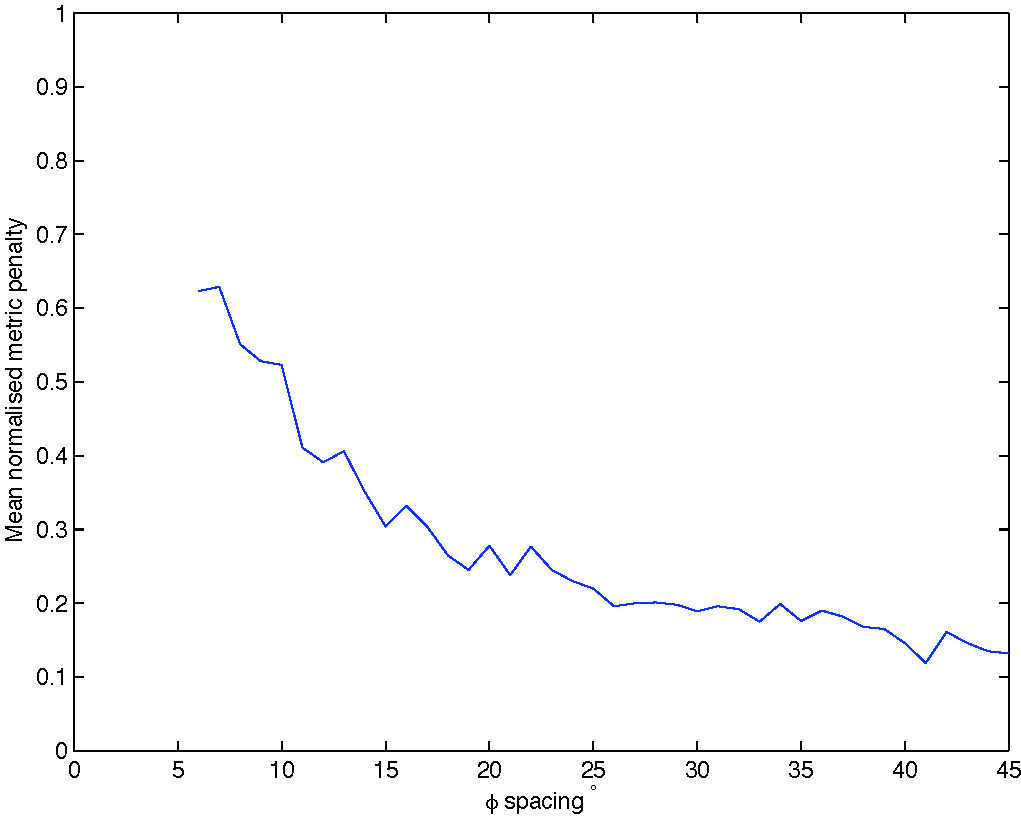
\includegraphics[scale=0.5]{figures/phi_spacing_45a.pdf}
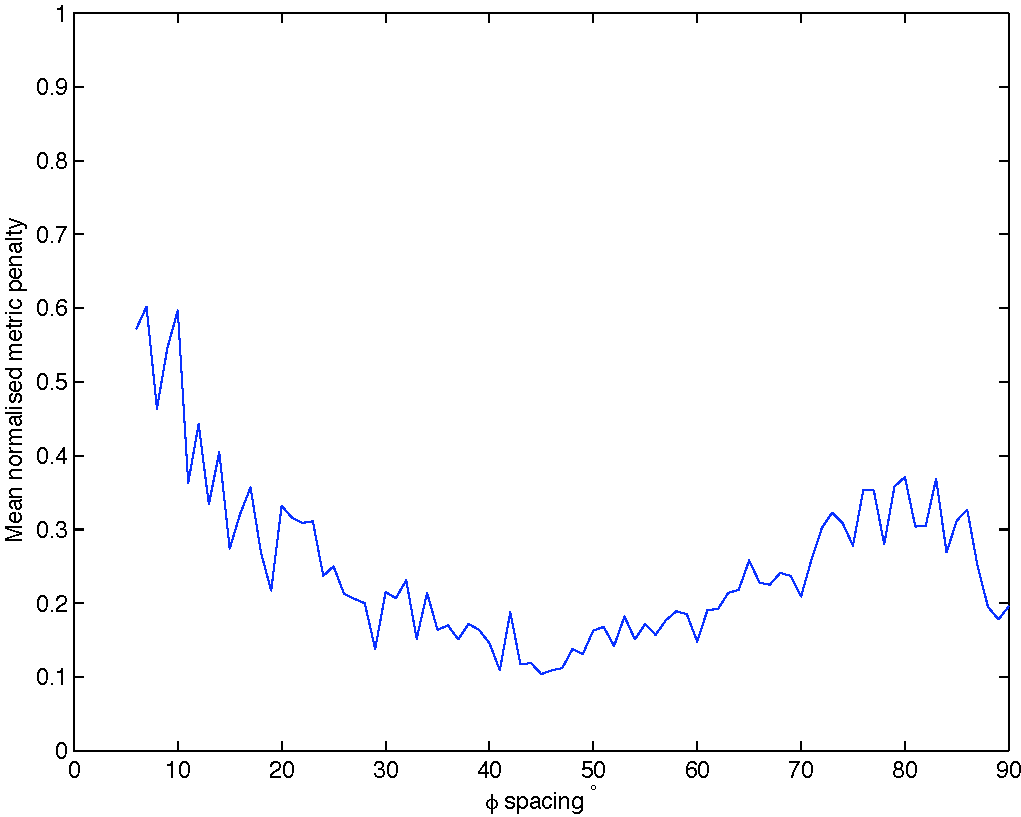
\includegraphics[scale=0.5]{figures/phi_spacing_90a.pdf}

\subsection{Integration}
\begin{itemize}
\item{Integrate with lattice constraints applied}
\item{Integrate to corners of detector}
\item{If good reason, repeat integration e.g. with results of postrefinement}
\item{Perform postrefinement in P1, assumed lattice - may reject lattice,
feed back to indexing}
\item{At the end of this we have LATTICE}
\item{If XDS, includes iterative elimination of outliers in CORRECT step}
\end{itemize}

\subsection{Scaling}
\begin{itemize}
\item{Compare results of pointless with remaining allowed lattices:
\begin{itemize}
\item{If agree, proceed}
\item{If lattice not allowed, consider next solution}
\item{If solution lower symmetry than lattice, reject and return to indexing}
\end{itemize}
}
\item{Ensure conclusions consistent}
\item{Now have corrrect LAUE GROUP}
\item{Ensure consistent setting / origin choice}
\item{Place data into data collection order}
\item{Analyse absences to decide likely SPACE GROUPs}
\item{Decide scaling model\footnote{For XDS use not corrections in CORRECT,
apply all corrections in XSCALE}}
\end{itemize}

\subsection{Merging and analysis}
\begin{itemize}
\item{If using XDS for integration and XSCALE for scaling, data still merged
with SCALA / AIMLESS}
\item{Resolution limits calculated from the intensities, not program output}
\item{``Downstream'' analysis (e.g. TRUNCATE and SFCHECK) identical}
\item{Working on scaling data direct from XDS with AIMLESS}
\end{itemize}

\section{What decisions were made?}

\subsection{Decisions: Indexing - LABELIT}
{\small
\begin{verbatim}
Solution  Metric fit  rmsd  #spots  crystal_system   unit_cell 
:)   9     0.2097 dg 0.327    533    tetragonal tP   42.32  42.32  39.28  ...
:)   8     0.2097 dg 0.364    541  orthorhombic oP   39.29  42.28  42.33  ...
:)   7     0.2097 dg 0.300    519    monoclinic mP   39.26  42.32  42.32  ...
:)   6     0.1950 dg 0.299    523    monoclinic mP   39.26  42.33  42.31  ...
:)   5     0.1307 dg 0.411    523  orthorhombic oC   59.71  59.91  39.31  ...
:)   4     0.1307 dg 0.412    524    monoclinic mC   59.91  59.71  39.31  ...
:)   3     0.0937 dg 0.429    524    monoclinic mC   59.71  59.91  39.30  ...
:)   2     0.1010 dg 0.298    512    monoclinic mP   42.27  39.31  42.32  ...
:)   1     0.0000 dg 0.291    509     triclinic aP   39.31  42.26  42.32  ...
\end{verbatim}
}

\subsection{Decisions: Indexing - IDXREF}
{\small
\begin{verbatim}
 *  31        aP          0.0      39.1   42.1   42.1  90.0  90.0  89.9
 *  44        aP          0.1      39.1   42.1   42.1  90.0  90.0  90.1
 *  34        mP          0.7      39.1   42.1   42.1  90.0  90.1  90.0
 *  20        mC          0.7      59.6   59.6   39.1  90.1  90.1  90.0
 *  33        mP          0.8      39.1   42.1   42.1  90.0  90.1  90.0
 *  25        mC          0.9      59.6   59.6   39.1  89.9  90.1  90.0
 *  35        mP          1.7      42.1   39.1   42.1  90.0  90.0  90.1
 *  23        oC          1.7      59.6   59.6   39.1  89.9  90.1  90.0
 *  32        oP          1.8      39.1   42.1   42.1  90.0  90.0  90.1
 *  21        tP          1.9      42.1   42.1   39.1  90.0  90.1  90.0
    10        mC         79.5      57.5   57.4   42.1  90.0  90.0  94.2
    13        oC         79.9      57.4   57.5   42.1  90.0  90.0  85.8
    14        mC         79.9      57.4   57.5   42.1  90.0  90.0  85.8
\end{verbatim}
}

\subsection{Decisions: Testing lattice choice}
\begin{itemize}
\item{Perform postrefinement (MOSFLM and XDS) in P1 and putative lattice}
\item{Compare R.M.S. deviation of observed / predicted centres}
\item{Results comparable $\rightarrow$ lattice probably OK}
\item{Results worse with lattice constraints $\rightarrow$ lattice probably
wrong}
\end{itemize}

\subsection{Decisions: Testing lattice choice 1}
{\small
\begin{verbatim}
 REFINED PARAMETERS:  DISTANCE BEAM ORIENTATION CELL AXIS                   
 USING   27389 INDEXED SPOTS
 STANDARD DEVIATION OF SPOT    POSITION (PIXELS)     1.28
 STANDARD DEVIATION OF SPINDLE POSITION (DEGREES)    0.23
...
 UNIT CELL PARAMETERS     42.180    42.183    39.236  90.002  89.989  89.986
 E.S.D. OF CELL PARAMETERS  1.8E-02 4.3E-02 1.5E-02 1.4E-02 1.0E-02 2.9E-02
 SPACE GROUP NUMBER      1
\end{verbatim}
}

\subsection{Decisions: Testing lattice choice 2}
{\small
\begin{verbatim}
 REFINED PARAMETERS:  DISTANCE BEAM ORIENTATION CELL AXIS                   
 USING   27378 INDEXED SPOTS
 STANDARD DEVIATION OF SPOT    POSITION (PIXELS)     1.29
 STANDARD DEVIATION OF SPINDLE POSITION (DEGREES)    0.23
...
 UNIT CELL PARAMETERS     42.187    42.187    39.242  90.000  90.000  90.000
 E.S.D. OF CELL PARAMETERS  1.6E-02 1.6E-02 1.2E-02 0.0E+00 0.0E+00 0.0E+00
 SPACE GROUP NUMBER     75
\end{verbatim}
}

\subsection{Decisions: Lattice observations}
\begin{itemize}
\item{Selecting lattice from indexing safe, as tested and challenged}
\item{However strong argument for performing all processing in P1:
\begin{itemize}
\item{Processing only performed once}
\item{Incorrect constraints cannot break things}
\item{Results generally comparable}
\end{itemize}
}
\item{This is on the to-do list...}
\end{itemize}

\subsection{Resolution limits - default criteria}
\begin{itemize}
\item{Merged $\frac{I}{\sigma_I} > 2$}
\item{Unmerged $\frac{I}{\sigma_I} > 1$}
\item{Control with -misigma, -isigma}
\end{itemize}

\subsection{Resolution limits - why unmerged $\frac{I}{\sigma_I} > 1$?}
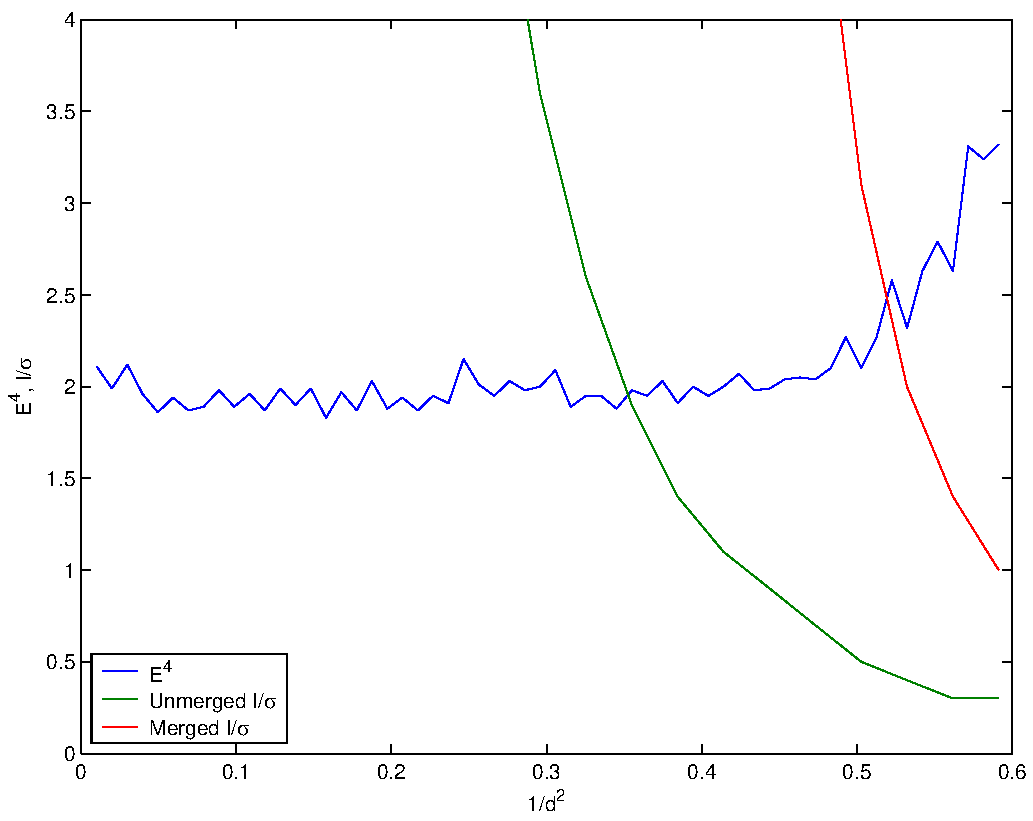
\includegraphics[scale=0.5]{figures/plat-13A-z4.pdf}
\footnote{90-fold multiplicity data from Ed Mitchell @ ESRF}
Though resolution limits to need to be revisited...

\section{Comments}

\subsection{Which options work best?}
\begin{itemize}
\item{It depends ...}
\item{... try for yourself!}
\item{Sometimes -2d (MOSFLM / SCALA) works better, sometimes -3d (XDS etc.)}
\item{Run both - compare results, make up your own mind}
\item{Hint for small molecule: -3dii -small\_molecule}
\item{-3d often works better for very fine $\phi$ sliced Pilatus data}
\end{itemize}

\section{Conclusions}

\subsection{Conclusions}
\begin{itemize}
\item{System available which can reduce your data on your behalf}
\item{Relies on your software: MOSFLM / LABELIT / CCP4 / XDS}
\item{Handles complex strategies so use them}
\item{Works on Windows / OS X / Linux / laptop / workstation / cluster}
\item{Best way to learn data reduction is to teach it}
\item{Computer is very dim but diligent pupil}
\item{Have a go yourself, or feel free to contribute to xia2}
\end{itemize}

\subsection{Getting xia2}
\begin{itemize}
\item{Blog: xia2.blogspot.com}
\item{Code: xia2.sf.net}
\item{List: xia2-list@lists.sourceforge.net}
\end{itemize}

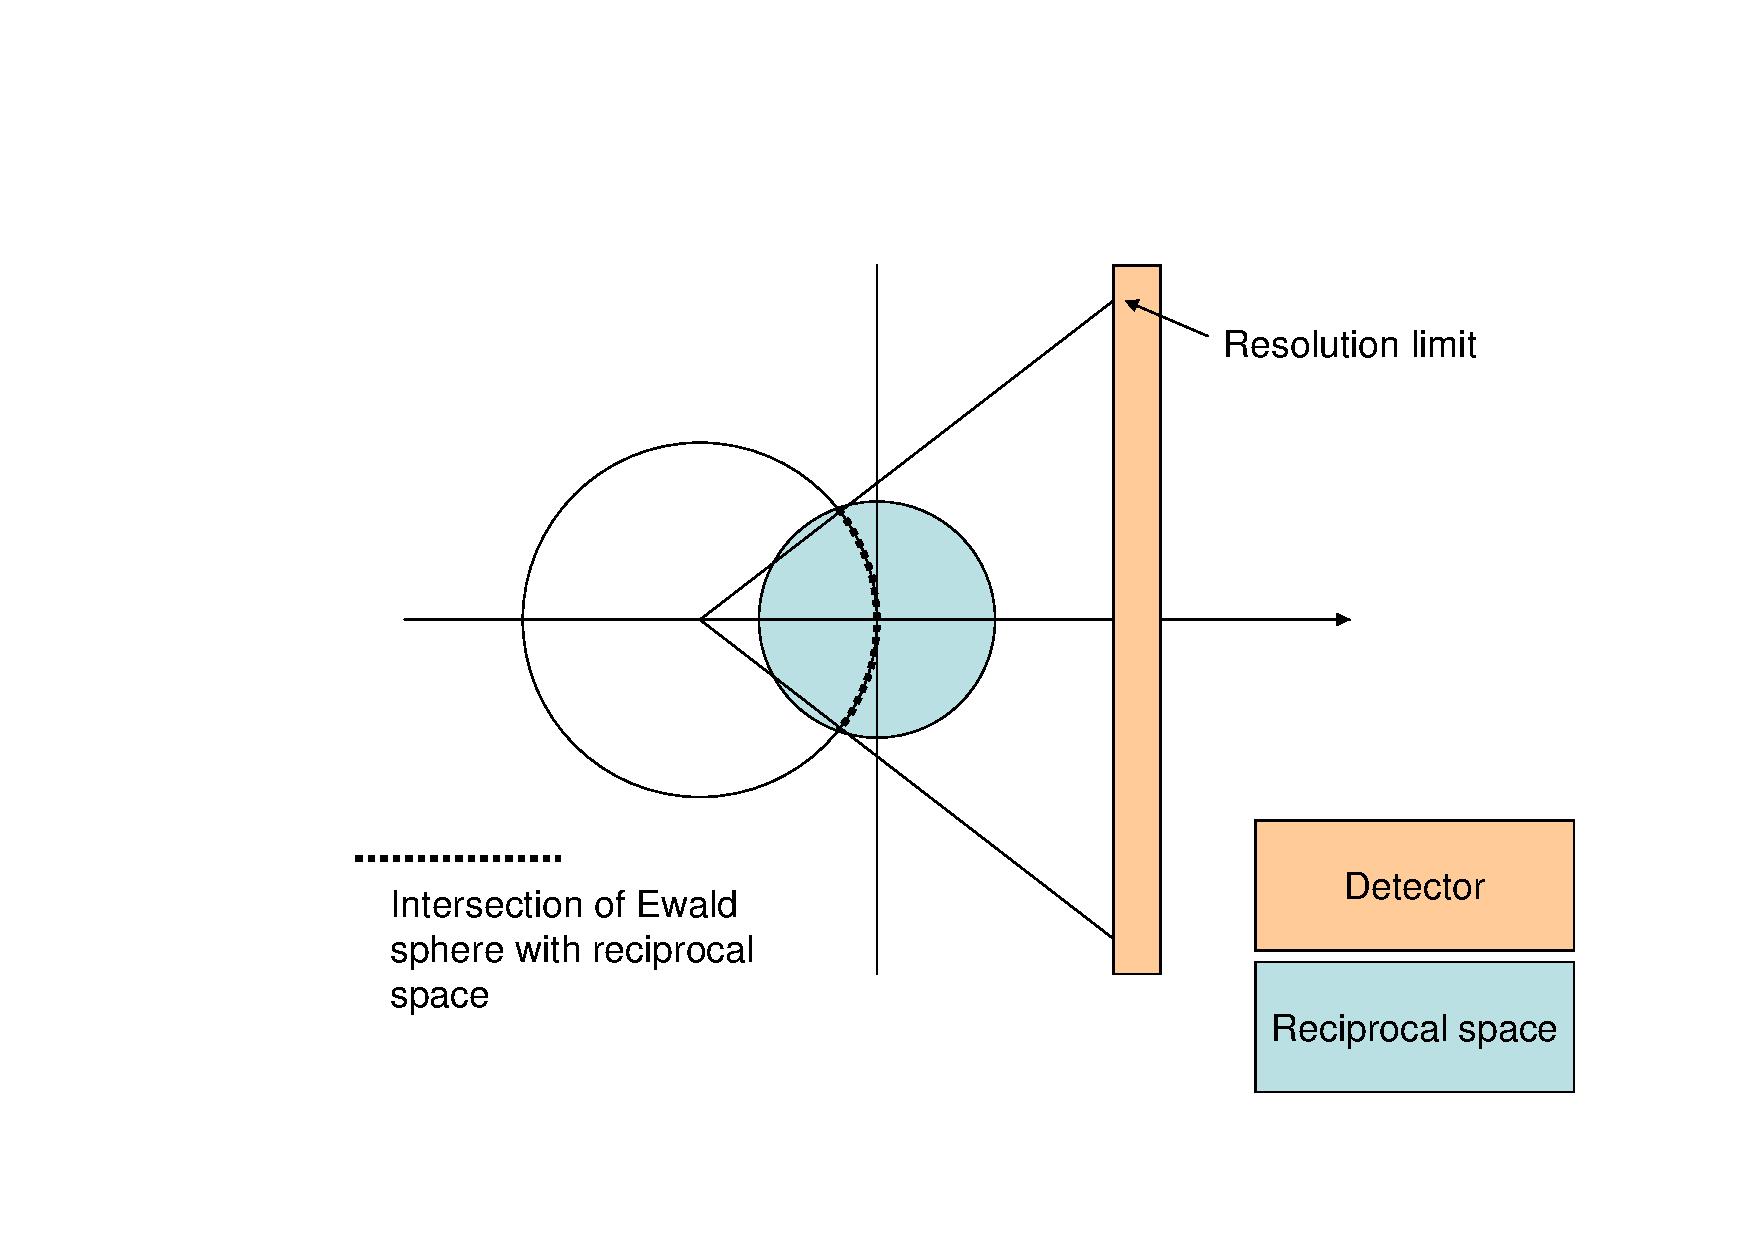
\includegraphics[scale=0.5]{figures/EwaldExplain.pdf}
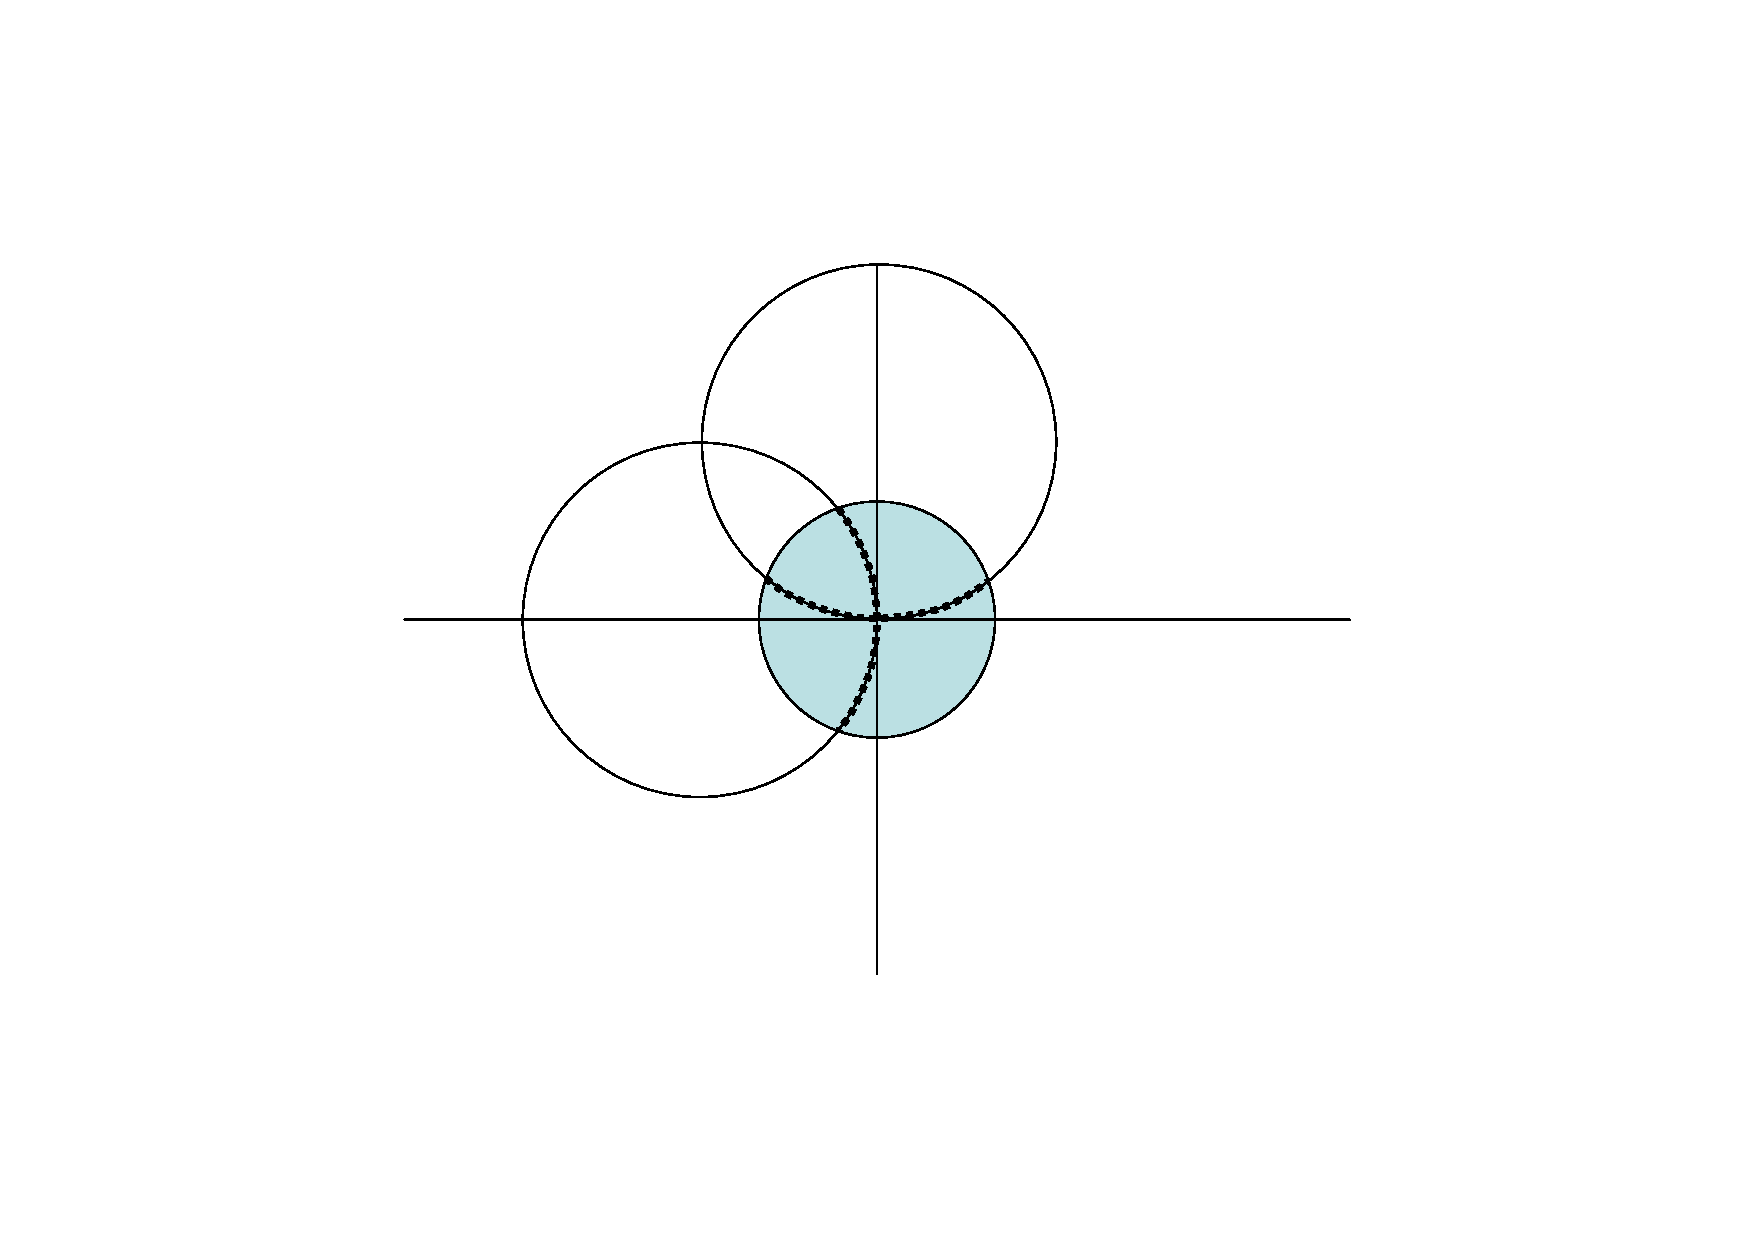
\includegraphics[scale=0.5]{figures/Ewald2Image.pdf}
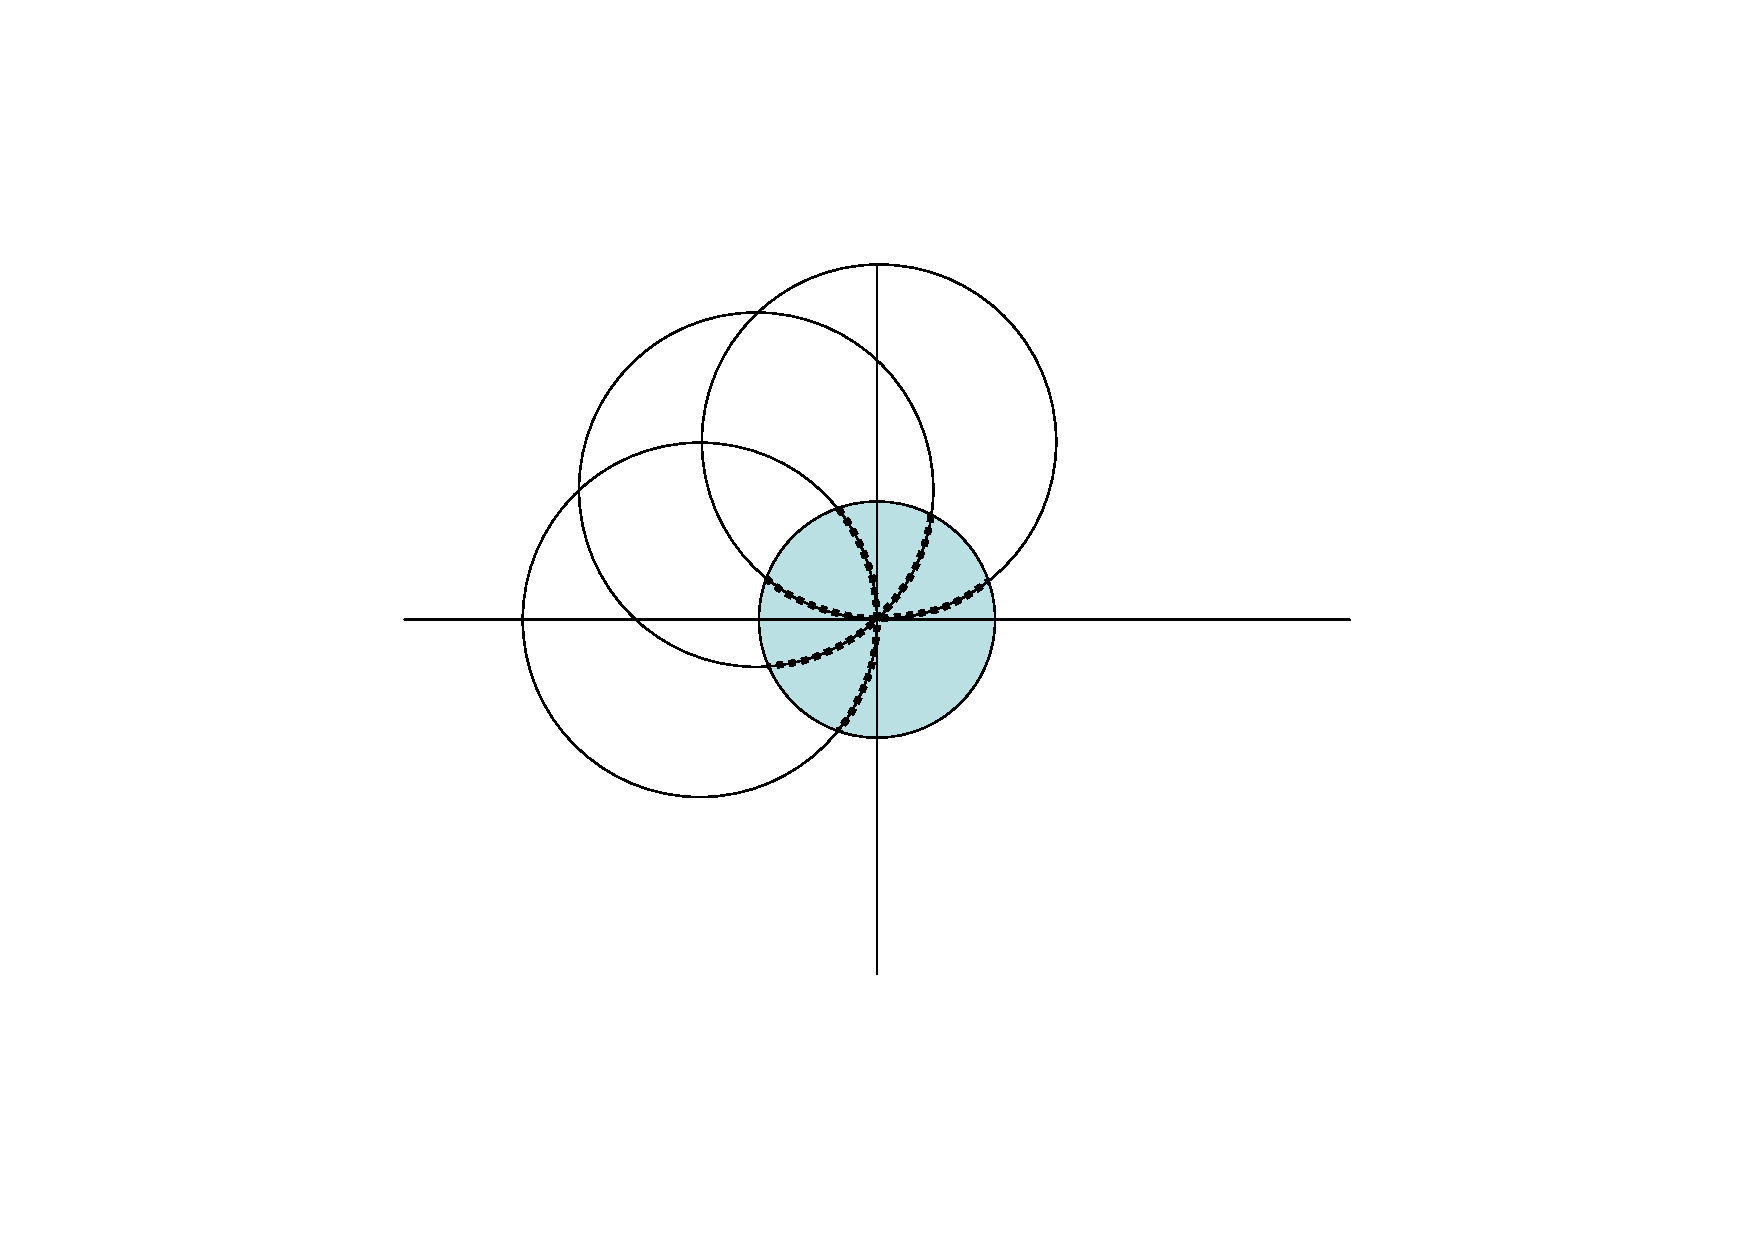
\includegraphics[scale=0.5]{figures/Ewald3Image.pdf}
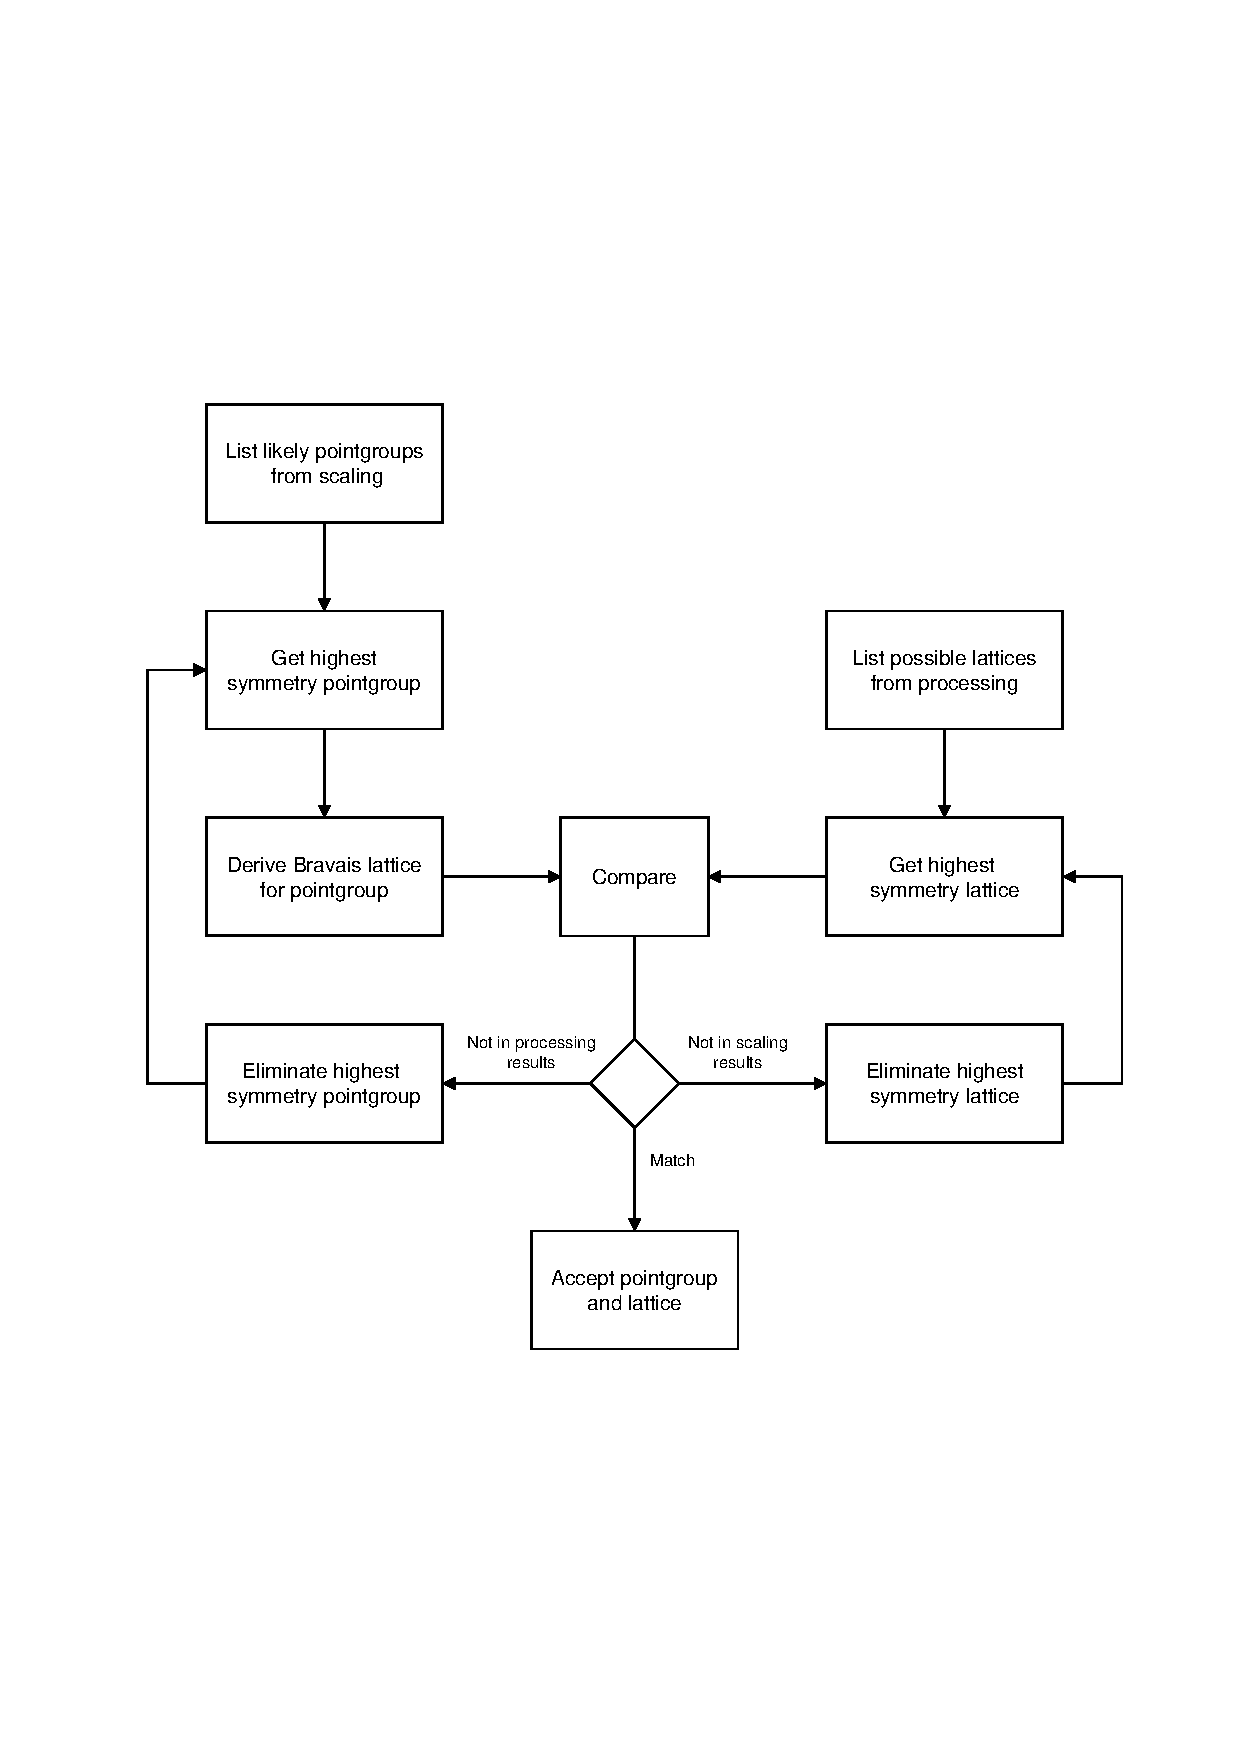
\includegraphics[scale=0.5]{figures/scaling-step-1.pdf}
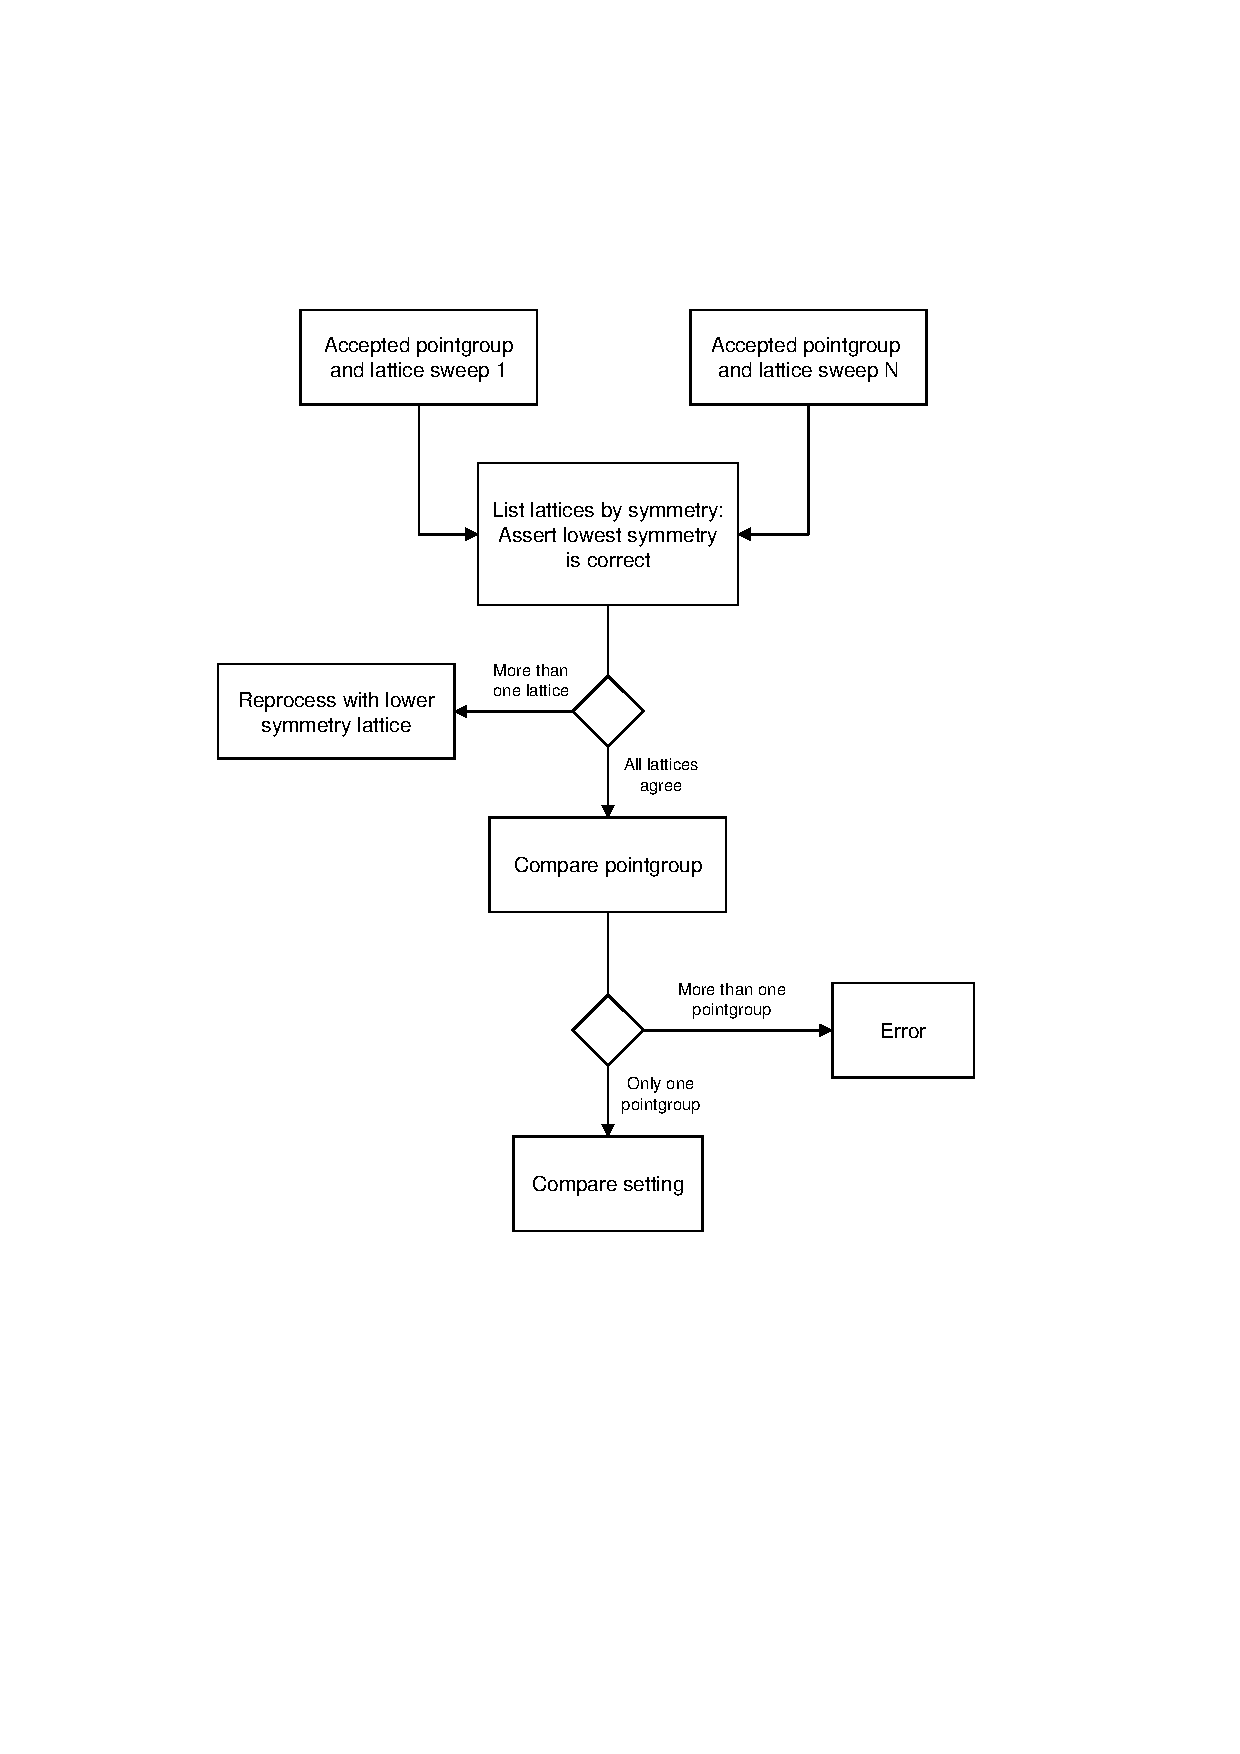
\includegraphics[scale=0.5]{figures/scaling-step-2.pdf}
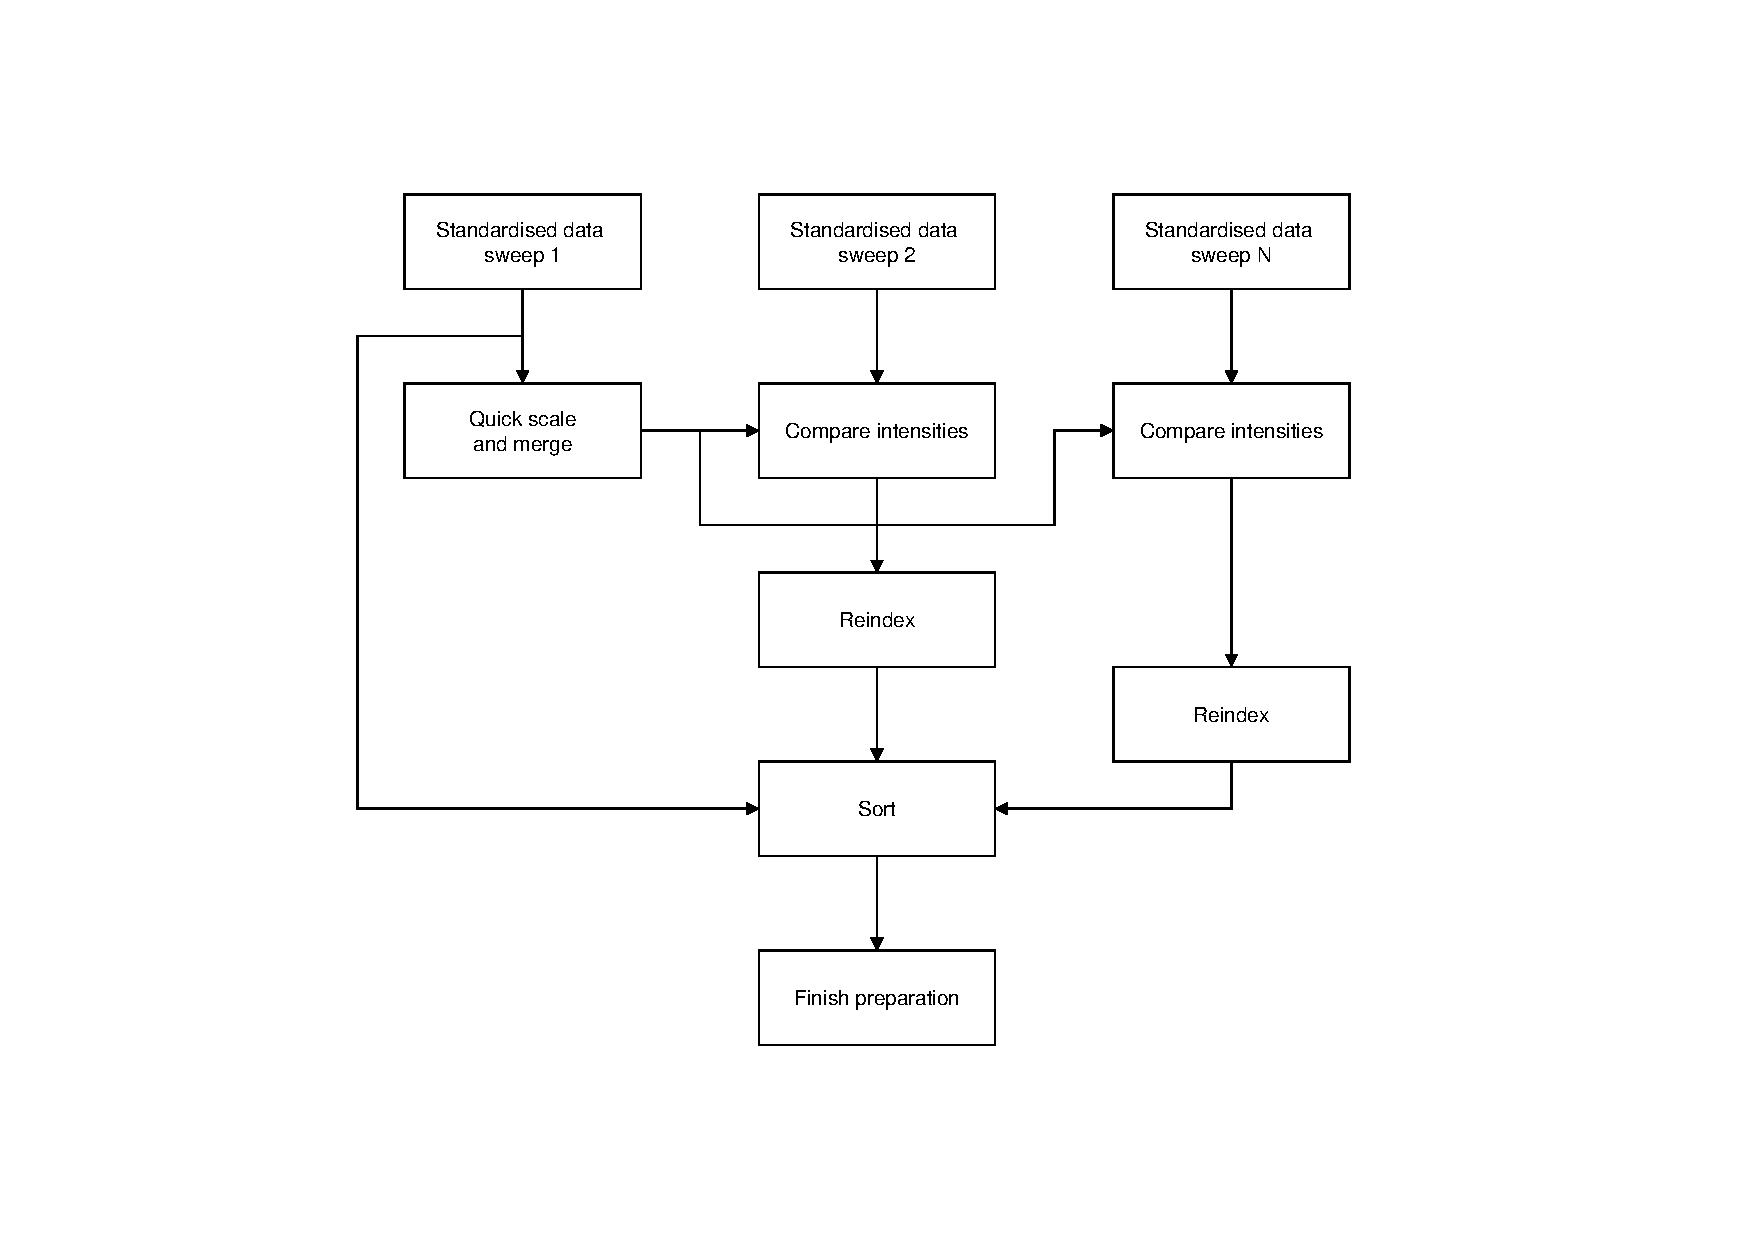
\includegraphics[scale=0.5]{figures/scaling-step-3.pdf}

\end{document}
